\documentclass[dvipdfmx,a4paper]{jsarticle}%pLatexでコンパイルしてください
\usepackage{ml4.2}  
\begin{document}
\maketitle
\vspace{-0.4cm}
\begin{figure}[H] 
  \centering
  \begin{tikzpicture}[remember picture, overlay]
      \node[anchor=north east] at (current page.north east) {
          \includegraphics[width=2cm]{pics/ml4.2.png} 
      };
      \node[anchor=north east, yshift=-2cm] at (current page.north east) {PDF版はここ$\uparrow$};
  \end{tikzpicture}
  \label{fig:my_label}
\end{figure}
\section{\texttt{Steepest Descent}(最急降下方向法)}
\thispagestyle{plain}
\noindent
小さなステップ幅 \ruby{\raisebox{2pt}{$\eta$}}{エータ}$>0$ を与えられたとき,
点 \(x^0\) において関数 \(f:\mathbb{R}^n\to\mathbb{R}\) をもっとも減少させる
単位ベクトル \(\nu\) を求めたい。

テイラー展開の 1 次近似より,
\[
 f(x^0+\eta \nu) - f(x^0)
   = \eta \langle \nabla f(x^0), \nu\rangle + o(\eta^2)
 \approx \eta \langle \nabla f(x^0), \nu\rangle.
\]

スカラー積に対するCauchy-Schwarzの不等式\footnotemark[1] $ |\langle a, b \rangle| \le \|a\| \|b\|\quad (a,b\in \mathbb{R}^n) $ から
\footnotetext[1]{証明はAppendixの\ref{convolution-proof}を参考してください。}
\[
 -\|\nabla f(x^0)\|\cdot\|\nu\| \le
 \langle \nabla f(x^0), \nu\rangle
 \le \|\nabla f(x^0)\|\cdot\|\nu\|
 \quad (\|\nu\|=1)
\]
であり,最小値は
\[
 \nu^* = -\frac{\nabla f(x^0)}{\|\nabla f(x^0)\|}
\]
で達成される。

\begin{reidai}{$\nu^*$の証明}{f}
$\nu^* = -\frac{\nabla f(x^0)}{\|\nabla f(x^0)\|}$となる証明
\end{reidai}
\kai \\

\noindent
\begin{proof}
  ラグランジュの未定乗数法を用いて示す。
制約条件 \(\|\nu\|^2 - 1 = 0\)のもとで
\(\langle \nabla f(x^0), \nu\rangle\)を最小化する。
ラグランジュ関数を
\[ \mathcal{L}(\nu,\lambda)
 = \langle \nabla f(x^0), \nu\rangle
   + \lambda(\|\nu\|^2 - 1) \]
とおく。
次に$\mathcal{L}$の$\nu$に関する偏微分は$0$にする
\[ \frac{\partial \mathcal{L}}{\partial \nu}
 = \nabla f(x^0) + 2\lambda \nu = 0 \]
から
\[ \nu = -\frac{1}{2\lambda}\nabla f(x^0). \]
制約条件に代入して
\[ \|\nu\|^2 = \frac{1}{4\lambda^2}\|\nabla f(x^0)\|^2 = 1 \]
を得る。したがって
\[ \lambda = \pm \frac{1}{2}\|\nabla f(x^0)\| \]
最小値を与えるのは負号の場合であり,(\ie $\lambda = -\frac{1}{2}\|\nabla f(x^0)\|$),その$\lambda$を$\nu$に代入すると
\[ \nu^* = -\frac{\nabla f(x^0)}{\|\nabla f(x^0)\|} \]
\end{proof}
したがって関数値の最大変化は近似的に
\[
 f(x^0+\eta \nu^*) - f(x^0)
   =\eta \langle \nabla f(x^0), \nu^*\rangle\footnotemark[2] = -\eta \|\nabla f(x^0)\|
\]
\footnotetext[2]{幾何の視点から考えると、\(\langle \nabla f(x^0), \nu^*\rangle = \|\nabla f(x^0)\|\cdot\|\nu^*\|\cdot\cos\theta = -\|\nabla f(x^0)\|\)となる。ここで、\(\theta\)は\(\nabla f(x^0)\)と\(\nu^*\)のなす角であり、\(\nu^*\)は\(\nabla f(x^0)\)の反対方向を向いているため、\(\theta = \pi\)である。}
となる。ここで \(\eta\) を \emph{学習率 (learning rate)} と呼ぶ。\\

\noindent
大域的最小点 \(x^*\) の吸引域内の初期点 \(x^0\) から始めて,
次の反復を考える:
\[
 x^{n+1} = x^n + \eta \nu^* = x^n - \eta
 \frac{\nabla f(x^n)}{\|\nabla f(x^n)\|}.
\tag{4.2.3}
\]

このとき
\[
 f(x^{n+1}) - f(x^n)
 = -\eta \|\nabla f(x^n)\| < 0\quad (\because\eta>0, \|\nabla f(x^n)\| > 0)
\]
が成り立ち,目的関数は必ず減少する。
一方で
\(\|x^{n+1}-x^n\|=\eta>0\) で一定のため,
一般には列 $(x^n)_n$ は収束しない。

\begin{prop}[標準的な勾配降下法]
ステップ幅を
\[
 \eta_n = \delta \|\nabla f(x^n)\|
 \quad (\exists\delta>0)
\]
と仮定すると,反復式 (4.2.3) は
\[
 x^{n+1} = x^n - \delta \nabla f(x^n)
 \tag{4.2.4}
\]
となる。これは標準的な勾配降下法である。
\end{prop}
\begin{reidai}{同値証明}{解答}
  反復式 \((4.2.4)\) により定義される列 \((x^n)\) が収束することと,
勾配列 \(\nabla f(x^n)\) が \(0\) に収束することは同値である。\ie $(x^n)_n$ が収束すること$\overset{\text{iff}}{\Longleftrightarrow}\nabla f(x^n)\rightarrow 0\quad (x\rightarrow \infty)$ 
\end{reidai}
\kai \\


\begin{proof}
\begin{description}[font=\normalfont, leftmargin=2em]
\item[\(\Rightarrow \):]\quad
\((x^n)_n\) が収束すると仮定する。このとき
\[
 0
 = \lim_{n\to\infty} \|x^{n+1} - x^n\|
 = \delta \lim_{n\to\infty} \|\nabla f(x^n)\|
\]
が成り立つので,
\[
 \nabla f(x^n) \longrightarrow 0 \quad (n\to\infty)
\]
が従う。

\item[\(\Leftarrow\):]\quad
\(\nabla f(x^n) \to 0 \ (n\to\infty)\) を仮定する。
任意の \(p \ge 1\) に対し,三角不等式より
\[
 \begin{aligned}
  \|x^{n+p} - x^n\|
  &= \bigl\| (x^{n+p} - x^{n+p-1}) + \cdots + (x^{n+1} - x^n) \bigr\| \\[2mm]
  &\le \|x^{n+p} - x^{n+p-1}\|
      + \cdots
      + \|x^{n+1} - x^n\| \quad \footnotemark[3] \\[2mm]
  &= \delta \sum_{j=0}^{p-1} \bigl\| \nabla f(x^{n+j}) \bigr\|.
 \end{aligned}
 \footnotetext[3]{証明はAppendixの\ref{triangle-inequality}を参考してください。}
\]

したがって,
\[
 \lim_{n\to\infty} \|x^{n+p} - x^n\|
 \le
 \delta \sum_{j=0}^{p-1}
   \lim_{n\to\infty} \bigl\| \nabla f(x^{n+j}) \bigr\|
 = 0.
\]
よって \((x^n)_n\) はコーシー列\footnotemark[4]であり,したがって収束する。

\end{description}
\end{proof}
\footnotetext[4]{数列${a_n}$がコーシー列であるとは,$\displaystyle\lim_{n,m\to \infty} |a_n - a_m| = 0$\quad \ie 任意の \(\epsilon > 0\) に対して,ある \(N\) が存在して,\(m,n \ge N\) のとき \(\|x^m - x^n\| < \epsilon\) となる列のことをいう。}

\noindent
もし \(f\) が連続的に微分可能($fはC^1級$)であれば,$\nabla f: \mathbb{R}^n \to \mathbb{R}^n$ は連続関数である。したがって、
\(x^n\to x^*\) から
\(\nabla f(x^n)\to\nabla f(x^*)\) が従う。
これは最適性条件と一致している。




\begin{exm}{峡谷関数の例}
  関数
  \[
   f(x,y) = \frac12 y^2 - x,
   \quad (x,y)\in(0,1)\times(-2,2)
  \]
  を考える。これは\emph{峡谷状(Canyon Type)}のグラフをもち,
  点 \((1,0)\) で最小値をとる。
  勾配は
  \[
   \nabla f(x,y)^{\mathsf{T}}
   = \left(\frac{\partial f}{\partial x},
            \frac{\partial f}{\partial y}\right)
   = (-1,y)
  \]
  である。
  
  反復式 (4.2.4) は
  \[
   \begin{cases}
    x^{n+1} = x^n + \delta,\\[1mm]
    y^{n+1} = (1-\delta)y^n
   \end{cases}
  \]
  となり,任意の初期点 \((x^0,y^0)\) に対し
  \[
   x^n = x^0 + n\delta,\qquad
   y^n = (1-\delta)^n y^0
  \]
  と表せる\footnotemark[5]。
  \footnotetext[5]{数学的帰納法により、\\ $x^1 = x^0 + \delta,x^2 = x^1 + \delta = x^0 + 2\delta ,\cdots , x^n = x^0 + n\delta\\ y^1 = (1-\delta)y^0,y^2 = (1-\delta)y^1 = (1-\delta)^2y^0,\cdots , y^n = (1-\delta)^n y^0$}
  
  \noindent
  次に、\((y^n)_n\) が収束する $\overset{\text{iff}}{\Longleftrightarrow} \displaystyle\lim_{n\to\infty} (1-\delta)^n = 0$により、$|1-\delta| < 1\iff 0 < \delta < 2$である。\\
  この範囲で次の二つの挙動が区別される。
  \begin{enumerate}[label=(\roman*), leftmargin=2em]
  \item \(0<\delta<1\) のとき,$1-\delta \in (1,0)\implies |1 -\delta|<1\implies \displaystyle\lim_{n\to\infty} (1-\delta)^n = 0$。従って、 $(y^n)_n$は収束する。 $x^{n+1}-x^n=\delta\implies$ $(x^n)_n$ は公差 \(\delta\)の
        等差数列として増加する。\ie $x^n \le 1\implies x^n = x^0 +n\delta \le 1\implies n\le \dfrac{1-x^0}{\delta}\quad (\delta >0)\implies n = \lfloor\dfrac{1-x^0}{\delta}\rfloor \quad\footnotemark[6]$。図1の\textbf{a}を参照してください。
  \vspace{1em}
  \item \(1<\delta<2\) のとき, $1-\delta <0$と$|1-\delta|<1$より、\(y^n\) は符号を交互に変えながら
        \(0\) に振動収束する。これは峡谷の両側を行き来しながら
        谷底を行き過ぎる挙動に対応する。図1の\textbf{b}を参照してください。
  \end{enumerate}
  \footnotetext[6]{$\lfloor\dfrac{1-x^0}{\delta}\rfloor$ とは、$\dfrac{1-x^0}{\delta}$を超えない最大の整数である床関数。\textbf{例:} $\lfloor 3.7 \rfloor = 3, \lfloor -2.3 \rfloor = -3$}
\newpage
\begin{figure}[htbp]
    \centering
    %\vspace{-2cm}
    % ==========================
    % 图 a (左侧)
    % ==========================
    \begin{minipage}{0.45\textwidth}
        \centering
        \begin{tikzpicture}[scale=0.9, >=latex]
            % 定义参数
            \def\starty{3.5}
            \def\decay{0.75}
            \def\nsteps{6}
            \def\xscale{0.8}

            % 坐标轴
            \draw[->] (0,0) -- (5.5,0) node[above left] {$x$};
            \draw[->] (0,0) -- (0,4) node[below right] {$y$};

            % 绘制点和连线
            % 计算坐标并保存
            \foreach \i in {0,...,\nsteps} {
                \coordinate (P\i) at (\i*\xscale, {\starty*pow(\decay,\i)});
            }

            % 画线 (连接各点)
            \draw (P0) 
            \foreach \i in {1,...,\nsteps} {
                -- (P\i)
            };

            % 画点
            \foreach \i in {0,...,\nsteps} {
                \fill (P\i) circle (1.5pt);
            }

            % 标注 (x^n, y^n) - 大约在第5个点附近
            \node[above right] at (P5) {$(x^n, y^n)$};

        \end{tikzpicture}
        \vspace{0.5cm}
        
        \textbf{\large a}
    \end{minipage}%
    \hfill
    % ==========================
    % 图 b (右侧)
    % ==========================
    \begin{minipage}{0.45\textwidth}
        \centering
        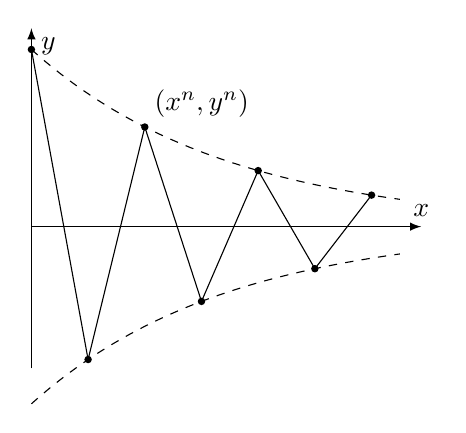
\begin{tikzpicture}[scale=0.9, >=latex]
            % 定义参数
            \def\starty{2.5}
            \def\decay{0.75}
            \def\nsteps{6}
            \def\xscale{0.8}

            % 坐标轴
            \draw[->] (0,0) -- (5.5,0) node[above] {$x$};
            \draw[->] (0,-2.0) -- (0,2.8) node[below right] {$y$};

            % 虚线包络线 (Envelope)
            \draw[dashed] plot[domain=0:5.2, samples=50] (\x, {\starty*pow(\decay,\x/\xscale)});
            \draw[dashed] plot[domain=0:5.2, samples=50] (\x, {-\starty*pow(\decay,\x/\xscale)});

            % 计算锯齿状的点
            \foreach \i in {0,...,\nsteps} {
                % (-1)^i * decay^i
                \coordinate (Q\i) at (\i*\xscale, {\starty*pow(-1,\i)*pow(\decay,\i)});
            }

            % 画折线
            \draw (Q0) 
            \foreach \i in {1,...,\nsteps} {
                -- (Q\i)
            };

            % 画点
            \foreach \i in {0,...,\nsteps} {
                \fill (Q\i) circle (1.5pt);
            }

            % 标注 (x^n, y^n) - 在上方包络线附近的某个点
            \node[above right] at (Q2) {$(x^n, y^n)$};

        \end{tikzpicture}
        \vspace{0.5cm}
        
        \textbf{\large b}
    \end{minipage}

    % 题注
    \caption{\textit{Iterations}: \textbf{a.} Case $0 < \delta < 1$. \textbf{b.} Case $1 < \delta < 2$.}
\end{figure}
\end{exm}
\appendix
\section{\\証明問題}

\subsection{\\Cauchy-Schwarzの不等式}\label{convolution-proof}
\begin{reidai}{Cauchy-Schwarzの不等式の証明}{解答}
$ a,b \in \mathbb{R}^n $ に対して、次の不等式を証明せよ。
\[ |\langle a, b \rangle| \le \|a\| \|b\| \]
等号成立の条件も述べよ。
\end{reidai}
\kai \\

\noindent
\begin{proof}
  $ a,b \in \mathbb{R}^n $ に対して、$ t \in \mathbb{R} $ とすると、次の式が成り立つ。
  \[
    0 \leq \|a - t b\|^2 = \langle a - t b, a - t b \rangle = \|a\|^2 - 2t \langle a, b \rangle + t^2 \|b\|^2
  \]
  右辺は $ t $ に関する二次式であり、常に非負であるため、判別式$\Delta\le 0$が必要がある。すなわち、
  \[
    (-2 \langle a, b \rangle)^2 - 4 \|b\|^2 \|a\|^2 \leq 0
  \]
  これを整理すると、Cauchy-Schwarzの不等式が得られる。
  \[
    |\langle a, b \rangle| \leq \|a\| \|b\|
  \]
  等号成立の条件は、$ a $ と $ b $ が線形従属である場合、すなわち、あるスカラー $ k\in T\subset \{\mathbb{R}\cup \mathbb{C}\} $ が存在して $ a = k b $ または $ b = k a $ が成り立つ場合である。

\end{proof}
\newpage
\subsection{三角不等式の証明}\label{triangle-inequality}
\begin{reidai}{三角不等式の証明}{解答}
  任意のベクトル $ a, b \in \mathbb{R}^n $ に対して、次の不等式を証明せよ。
  \[
    \|a + b\| \leq \|a\| + \|b\|
  \]
\end{reidai}
\kai \\

\noindent
\begin{proof}
  ベクトル $ a, b \in \mathbb{R}^n $ に対して、次の式が成り立つ。
  \begin{align*}
    \|a + b\|^2 &= \langle a + b, a + b \rangle \\
    &= \|a\|^2 + 2\langle a, b \rangle + \|b\|^2 \\
    &\leq \|a\|^2 + 2\|a\|\|b\| + \|b\|^2 \quad (\text{Cauchy-Schwarzの不等式より}) \\
    &= (\|a\| + \|b\|)^2
  \end{align*}
  両辺の平方根を取ると、三角不等式が得られる。
  \[
    \|a + b\| \leq \|a\| + \|b\|
  \]
\end{proof}


\end{document}